\chapter{Power Plant Cost Model Results}\label{ch6:cm_results}

Chapter \ref{ch4:cm_prep} outlined the cost modeling strategy for a hypothetical 5 MW expansion project of the Lightning Dock power plant in Animas Valley, NM. This chapter reviews the results of the different model approaches, explores insights gained from those models, and describes how this approach mitigates risks associated with geothermal production.

\section{Static Model}
\label{ch6:static_mod}

\subsection{Model Selection}
\label{ch6:static_select}

Section \ref{ch4:cm_rev} described the use of brine effectiveness in the cost model for determining the power output of a binary cycle plant for a given production temperature and flow rate. This formulation provides a choice of how to manage the cost model mechanics due to a trade-off between plant capacity and flow rate for a given brine effectiveness (Equation \ref{eq:cm_rev}).

In addition, installation of the Lightning Dock expansion can take place over a variety of different deployment schedules due to the modularity of the system. Rather than drill ten wells and install five binary cycle plants all at once, delaying aspects of the installation can be financially beneficial and less of an initial risk for the project.  

Figure \ref{fig:static_model_compare} shows the results for the pre-set capacity and pre-set flow rate static models for sixty (60) installation schedule permutations. The pre-set capacity model results in project losses of \$20 million or more for all tested installation options. On the other hand, the fixed flow-rate model only drops below \$0 NPV for a handful of project plans, achieving \$3.7 million NPV for the case marked with a red diamond where three (3) modules are installed up front and two (2) additional ones go live after a year of operation. Based on these results, all cost models used in the rest of this analysis apply a fixed flow rate per production well and derive the aggregate electricity generation numbers based on the temperature of the produced brine.

\begin{figure}[!htp]
\centering
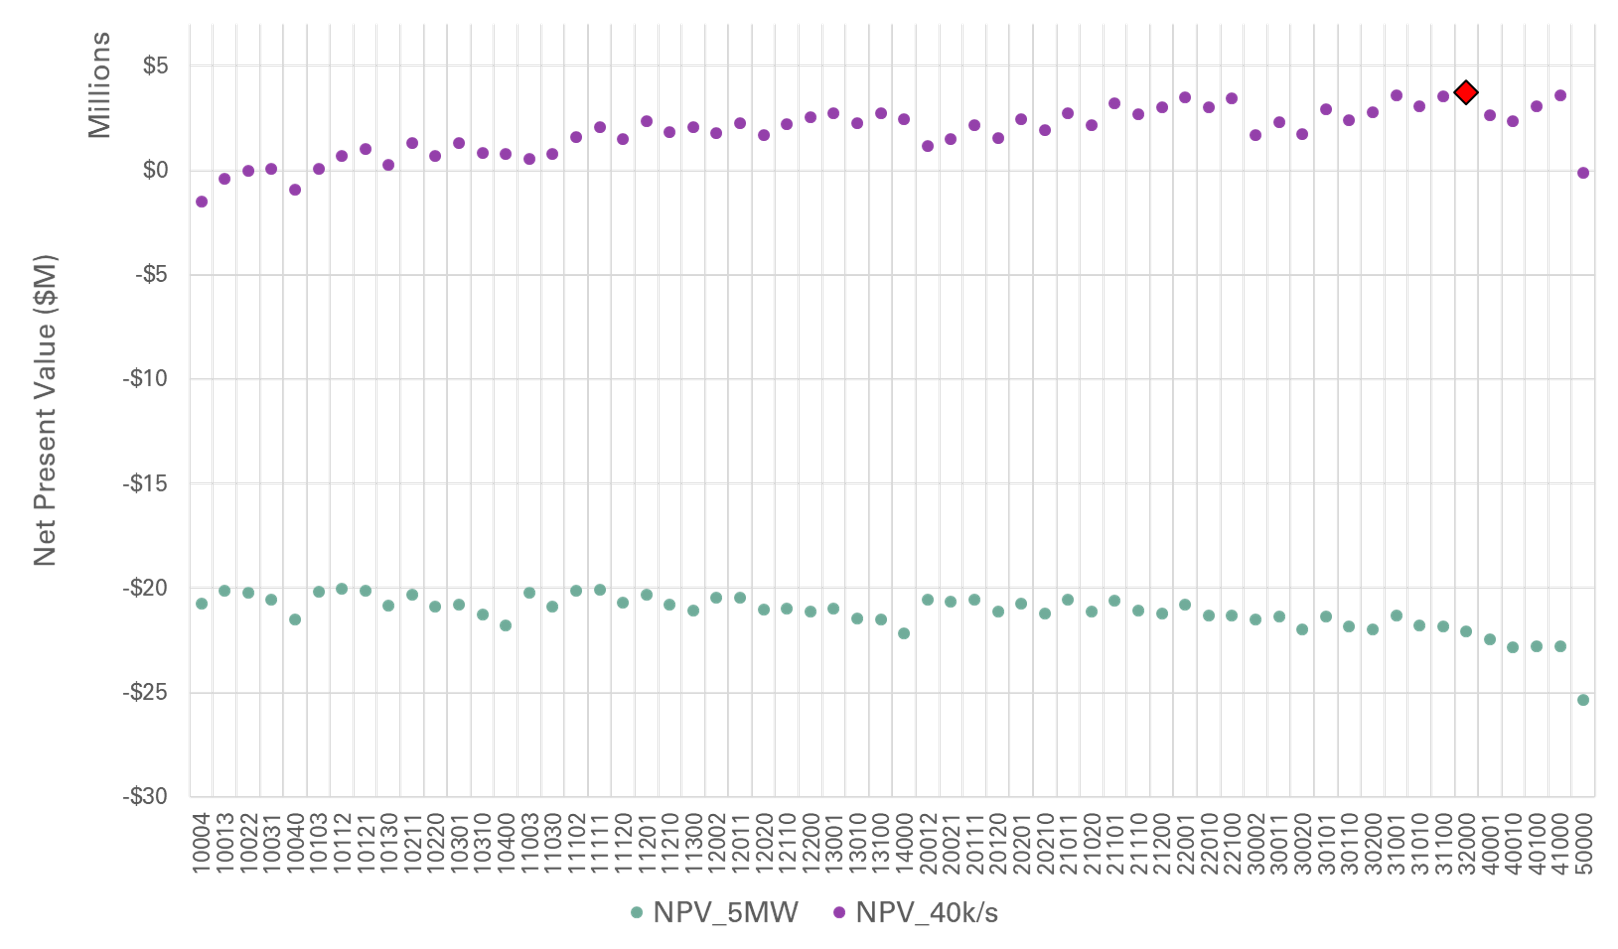
\includegraphics[width=.98\textwidth]
{templates/images/Figure-Static_Model_Construction.png}
\caption[Static cost model comparison]{Static cost model comparison between pre-set aggregate capacity (5 MW target, green) and pre-set flow rate per production well (40 kg/s, purple), plotted against module installation schedule. Both models deploy five modules in all schedule permutations involving up to a five-year period. The red diamond marks the optimal model and power plant expansion plan.}
\label{fig:static_model_compare}
\end{figure}

\subsection{Construction Optimization}
\label{ch6:static_schedule}

Lifting the fixed-capacity requirement changes the production potential for each power plant module. Based on the production parameters defined in Section \ref{ch4:cm_params}, each module can now generate 2.1 MW. Since this is a hypothetical case study with Climeon modules used as an analog only, further modeling uses this value with the caveat that future efforts confirm its viability as the modular power plant technology continues to evolve.

The updated power production per module reduces the required module count to a total of three (3) modules based on the original expansion target of $\approx$5 MW. Table \ref{tab:static_optimization} revisits the installation schedule grid search exercise to determine the optimal project plan under these circumstances. At an NPV of \$1.0 million, the best option deploys two (2) modules initially and adds an additional one (1) at the end of the first year. In order to standardize cost models for direct comparison, this installation plan is used for all cost models throughout the rest of this analysis.

\begin{table}[!htp]%{R}{0.4\linewidth}
\centering
\begin{tabular}{|c|c|c|c|}
\hline
\textbf{Year 0} & \textbf{Year 1} & \textbf{Year 2} & \textbf{NPV (\$M)} \\ \hline
3 & 0 & 0 & -\$1.1 \\ \hline
1 & 0 & 2 & -\$0.3 \\ \hline
1 & 1 & 1 & \$0.5 \\ \hline
1 & 2 & 0 & \$0.6 \\ \hline
2 & 0 & 1 & \$0.6 \\ \hline
2 & 1 & 0 & \$1.0 \\ \hline
\end{tabular}
\caption[Static model module installation schedule]{Grid search for the optimal power plant installation schedule based on the static cost model. Values are in \$M, where M is million.}
\label{tab:static_optimization}
\end{table}

\subsection{Summary Statistics}
\label{ch6:static_stats}

As a deterministic cost model, Static model performance is measured strictly on calculated NPV. This will act as a benchmark value for the other cost models explored in the rest of this chapter.

\begin{table}[H]
\centering
\begin{tabular}{|l|c|}
\hline
\textbf{Static Model Statistics} & \textbf{\$M} \\ \hline
NPV & \$1.0 \\ \hline
\end{tabular}
\caption[Static model statistics]{Static model statistics. NPV is reported in \$M, where M is million.}
\label{tab:static_mod_stats}
\end{table}

\section{Probabilistic Model Metrics}

Monte Carlo simulation is applied to all of the probabilistic models to estimate the range of model behavior. For each model, results represent 2000 simulated runs where each realization defines a unique combination of variable values sampled from the PDFs reviewed in Section \ref{ch4:pdfs}. 

Common methods for evaluating a Monte Carlo ensemble include building a NPV histogram, constructing a \acrlong{cdf} (\acrshort{cdf} or target curve), and averaging the results together for \acrlong{enpv} (\acrshort{enpv}). Other interesting metrics for model comparison include standard deviation, individual percentiles, and direct comparison with the static model NPV (NPV$_{s}$). Standard deviation is the measure of how tightly the results cluster around the central value. Distributions with low standard deviations are sometimes referred to as robust distributions. P$_{50}$ marks the the median, and P$_{05}$ and P$_{95}$ define marginal percentiles for 5\% Value At Risk (VAR) and Value At Gain (VAG), respectively. Each of these measures is reported for the probabilistic model cases described below.

\section{Base Case Probabilistic Model}
\label{ch6:base_case}

The Base Case model mimics the Static model in form, but incorporates uncertainties in drilling \& completions costs, electricity pricing, geothermal gradient, reservoir temperature, and thermal drawdown rate to provide a more realistic forecast. No decision rules are included in this scenario. 

\subsection{Model Results}
\label{ch6:base_results}

At -\$4.8 million ENPV, the Base Case model predicts over 560\% lower project value than predicted with the Static model (Table \ref{tab:base_stats}). This result alone illustrates how probabilistic approaches can significantly differ from deterministic models that use most-likely or average values. Skewed system performance occurs even when variable distributions are balanced, which makes deterministic results both unrealistic and unreliable measures for decision-making \citep[p.\ 48-49]{de_neufville_flexibility_2011}. Here, unanticipated high-side (P$_{95}$ value of \$15.9 million) does exist, but the influence of the low-side (P$_{05}$ value of -\$28.2 million) dominates overall (Table \ref{tab:base_stats}).

The Base Case ensemble shows a symmetric, pseudo-Gaussian distribution of NPV results, with the exception of a long right tail capturing rare but very positive project outcomes (Figure \ref{fig:base_case_hist}). Figure \ref{fig:base_case_cdf} illustrates the target curve tracing cumulative probabilities for observed NPV values. The P$_{50}$ value of -\$3.9 million suggests the highly-negative values in the lower half of results pull the average (ENPV) further into negative project value territory. Cumulatively, $\approx60\%$ of the realizations end in a net loss for the project (Figure \ref{fig:base_case_cdf}). And at $\approx 3\times$ both the median and ENPV, standard deviation of NPV indicates this solution is not robust. 

\begin{figure}[!htp]
\centering
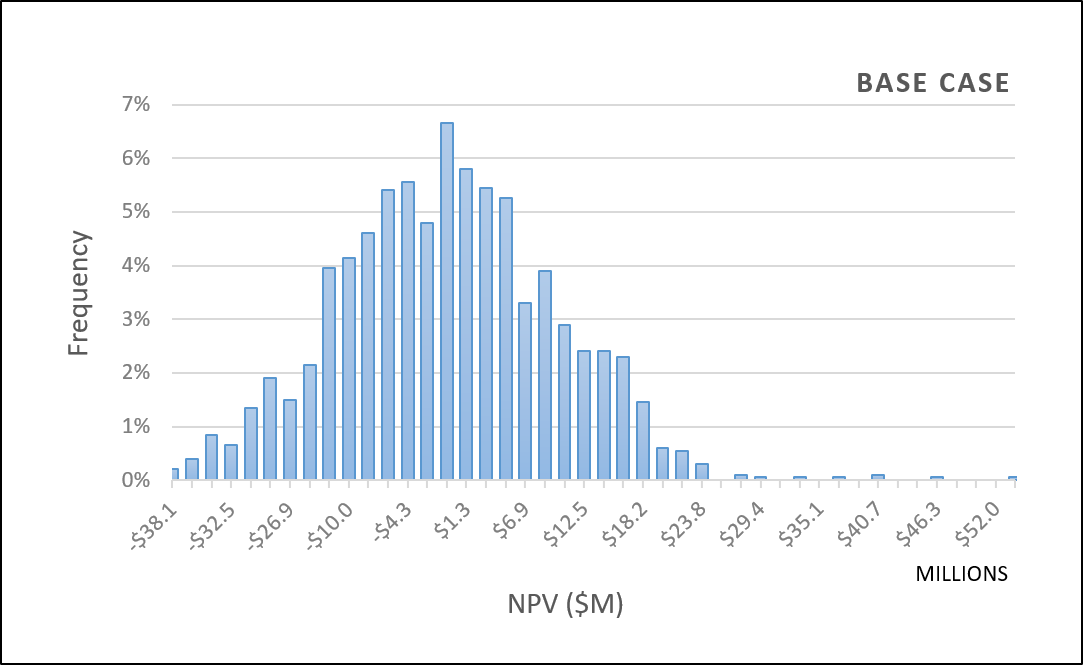
\includegraphics[width=.85\textwidth]{templates/images/Figure-Base_Case_Histogram.png}
\caption[Probabilistic Base Case histogram]{Base Case probabilistic cost model histogram illustrating the distribution of 2000 model realizations. NPV is reported in \$M, where M is million.}
\label{fig:base_case_hist}
\end{figure}

\begin{figure}[!htp]
\centering
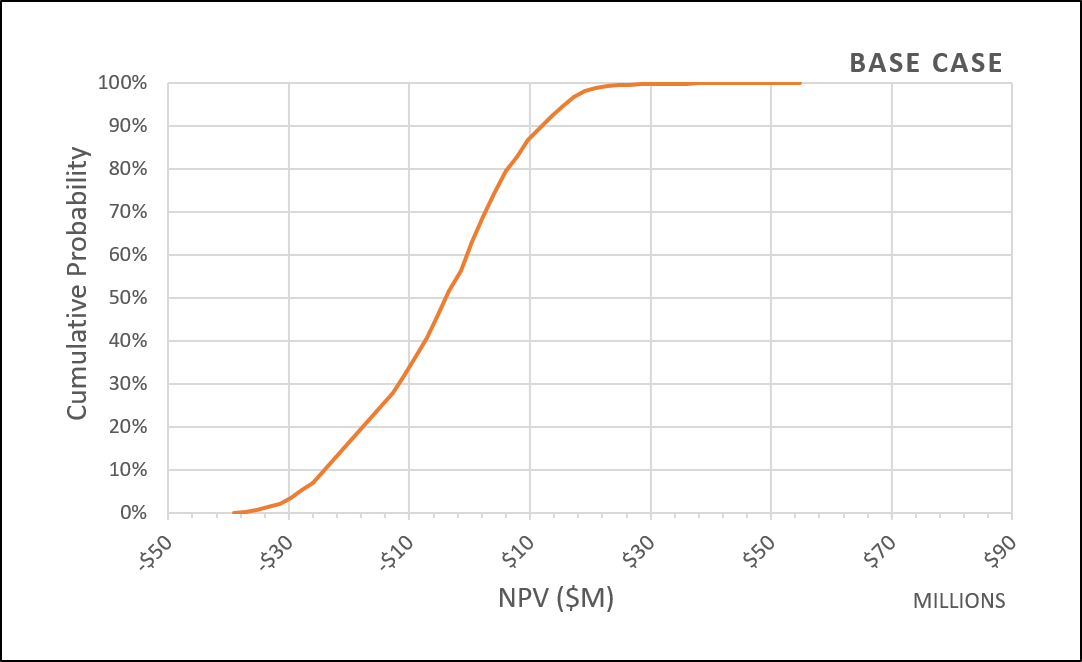
\includegraphics[width=.85\textwidth]{templates/images/Figure-Base_Case_CDF.png}
\caption[Probabilistic Base Case CDF]{Cumulative distribution function for the Base Case probabilistic cost model. The curve summarizes results from 2000 model realizations. NPV is reported in \$M, where M is million.}
\label{fig:base_case_cdf}
\end{figure}

All told, the Base Case results display both a negative ENPV and a high likelihood of project financial loss. Without a clear strategy for mitigating risk, this project would and should be rejected by a responsible portfolio manager.

\subsection{Summary Statistics}
\label{ch6:base_stats}

Table \ref{tab:base_stats} outlines key statistical measures summarizing the performance of the Base Case probabilistic cost model.

\begin{table}[H]
\centering
\begin{tabular}{|l|r|}
\hline
\textbf{Base Case Statistics} & N=2000 \\ \hline
ENPV & -\$4.8M \\ \hline
STD(NPV) & \$13.2M \\ \hline
P05 NPV & -\$28.2M \\ \hline
P50 NPV & -\$3.9M \\ \hline
P95 NPV & \$15.9M \\ \hline
\% Difference from NPV$_{s}$ & -565\% \\ \hline
\end{tabular}
\caption[Probabilistic Base Case statistics]{Base case probabilistic model statistics for 2000 model realizations. NPV is reported in \$M, where M is million. NPV$_s$ refers to the static model NPV, as reported in Table \ref{tab:static_mod_stats}.}
\label{tab:base_stats}
\end{table}

\section{Redevelop Case Probabilistic Model}

The Redevelop Case model extends the Base Case with a redevelopment plan for the geothermal field to counter thermal decline in the fluid pathways through the reservoir. The Redevelopment decision rule (Section \ref{ch4:dr_redevelop}) is triggered when thermal drawdown causes the produced brine to drop below a threshold temperature. As with the Base Case, model uncertainties include drilling \& completions costs, electricity pricing, geothermal gradient, reservoir temperature, and thermal drawdown rate.

\subsection{Model Results}
\label{ch6:redevelop_results}

Adding the Redevelopment rule improves the project ENPV by \$2.3 million over the Base Case, but it still remains negative at -\$2.5 million, 340\% below the Static model NPV. Redevelopment drilling costs come into play as the VAG (P$_{05}$ value of \$15.1 million) decreases slightly relative to the Base Case. But VAR (P$_{95}$ value of \$21.3 million) shows a larger difference, improving by nearly \$7 million over the Base Case (Table \ref{tab:redevelop_stats}). This clearly reflects the improved production and power sales possible by managing reservoir conditions.

Standard deviation of the ensemble distribution is less than observed for the Base Case, likely due to a narrower overall distribution without as many outliers in the tails (Figure \ref{fig:redevelop_case_hist}). The balance in distribution shape is reflected in the small difference (\$0.2 million) between ENPV and the P$_{50}$ result (Table \ref{tab:redevelop_stats}). Comparing the target curves between the Redevelop Case (Figure \ref{fig:redevelop_case_cdf}) and Base Case (Figure \ref{fig:base_case_cdf}), it becomes clear that the redevelopment flexibility does not address upside potential. Instead, it acts as a partial stop-gap on the worst case realizations of the model. The lower half of the curve tightens up, but there is little overall curve movement to the right to make the project more profitable.

\begin{figure}[!htp]
\centering
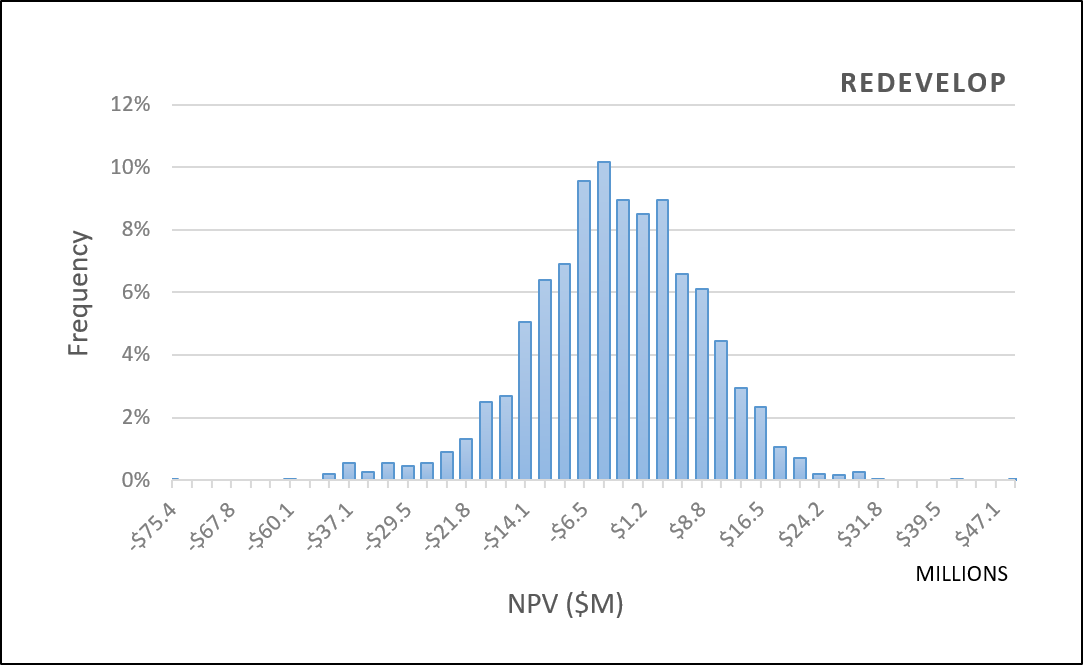
\includegraphics[width=.85\textwidth]{templates/images/Figure-Redevelop_Case_Histogram.png}
\caption[Probabilistic Redevelop Case histogram]{Redevelop Case probabilistic cost model histogram illustrating the distribution of 2000 model realizations. NPV is reported in \$M, where M is million.}
\label{fig:redevelop_case_hist}
\end{figure}

\begin{figure}[!htp]
\centering
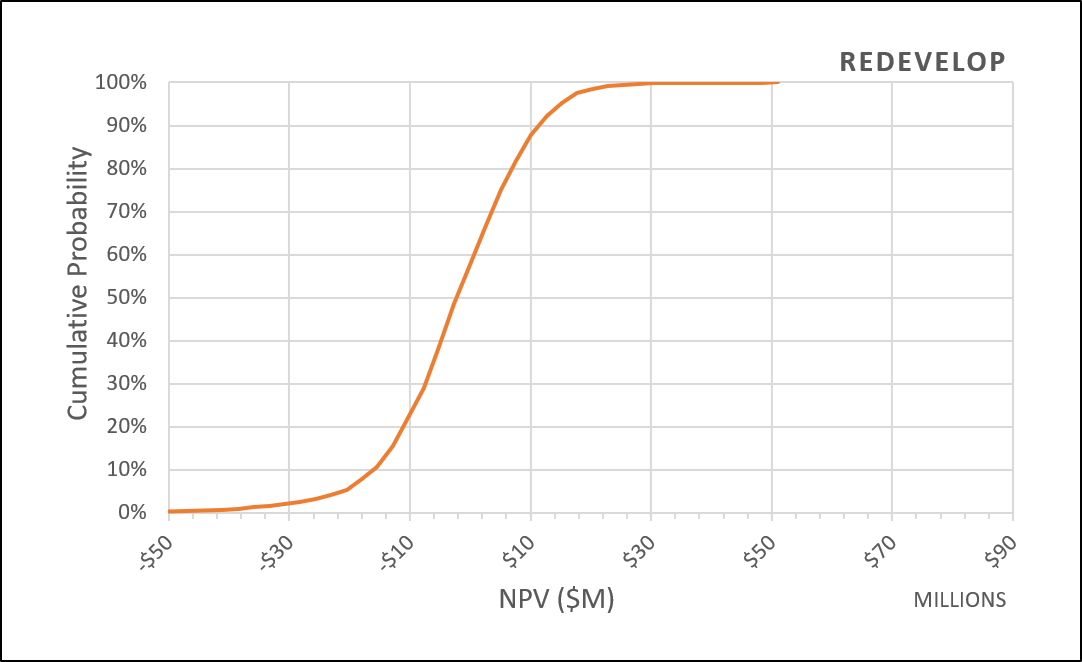
\includegraphics[width=.85\textwidth]{templates/images/Figure-Redevelop_Case_CDF.png}
\caption[Probabilistic Redevelop Case CDF]{Cumulative distribution function for the Redevelop Case probabilistic cost model. The curve summarizes results from 2000 model realizations. NPV is reported in \$M, where M is million.}
\label{fig:redevelop_case_cdf}
\end{figure}

As a brief caveat: the idea of periodic redevelopment for a geothermal field is not novel. In fact, many geothermal cost models include it as default behavior \citep[e.g.,\ ][]{entingh_volume_2006, freeman_system_2018}. Nevertheless, the analysis above illustrates why this design option should be included in geothermal operations to help mitigate the risk of high thermal drawdown rates --- as long as drilling costs are low enough to make it attractive. 

\subsection{Summary Statistics}
\label{ch6:redevelop_stats}

Table \ref{tab:redevelop_stats} outlines key statistical measures summarizing the performance of the Redevelop Case probabilistic cost model.

\begin{table}[H]
\centering
\begin{tabular}{|l|r|}
\hline
\textbf{Redevelop Case Statistics} & N=2000 \\ \hline
ENPV & -\$2.5M \\ \hline
STD(NPV) & \$11.7M \\ \hline
P05 NPV & -\$21.3M \\ \hline
P50 NPV & -\$2.3M \\ \hline
P95 NPV & \$15.1M \\ \hline
\% Difference from NPV$_{s}$ & -344\% \\ \hline
\end{tabular}
\caption[Probabilistic Redevelop Case statistics]{Redevelop case probabilistic model statistics for 2000 model realizations. NPV is reported in \$M, where M is million. NPV$_s$ refers to the static model NPV, as reported in Table \ref{tab:static_mod_stats}.}
\label{tab:redevelop_stats}
\end{table}

\section{Redevelop \& Grow Case Probabilistic Model}

The Redevelop \& Grow Case model builds on the Redevelop Case with a decision rule around increasing capacity (Section \ref{ch4:dr_grow}). Specifically, when electricity prices rise by an amount larger than the monitored threshold, more power plant modules are installed to capitalize on the increased prices and inferred demand. Like the other probabilistic models, values for drilling \& completions costs, electricity pricing, geothermal gradient, reservoir temperature, and thermal drawdown rate are directly sampled from probability distribution functions (Section \ref{ch4:pdfs}) as part of the Monte Carlo simulation.

\subsection{Model Results}
\label{ch6:grow_results}

Redevelop \& Grow model results use a field expansion amount of 25\% when the Grow Capacity decision rule is triggered. Assuming the PPA with the purchasing utility company is successfully renegotiated at the time of the expansion, this model results in a dramatic change in project value. ENPV is \$9.7 million, over \$12 million better than the Redevelop Case and over 800\% greater than Static model NPV (Table \ref{tab:grow_stats}). The case shows notable improvement in both Value at Risk and Value at Gain; P$_{05}$ shifts by more than \$7 million to -\$14.2 million, and P$_{95}$ leaps to \$38.2 million as power plant growth captures market potential.

\begin{figure}[!htp]
\centering
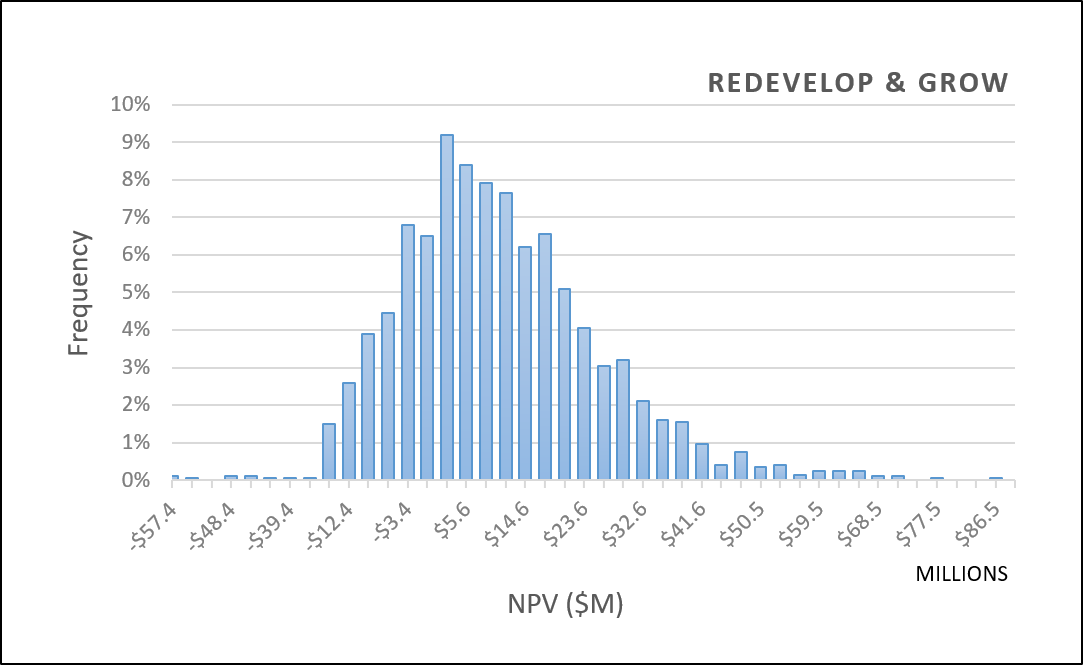
\includegraphics[width=.85\textwidth]{templates/images/Figure-Grow_Case_Histogram.png}
\caption[Redevelop \& Grow Case histogram]{Redevelop \& Grow Case probabilistic cost model histogram illustrating the distribution of 2000 model realizations. NPV is reported in \$M, where M is million.}
\label{fig:grow_case_hist}
\end{figure}

The histogram for Redevelop \& Grow skews noticeably to the left with a long tail of simulation runs marking high-value realizations of the model. Standard deviation of NPV increases compared to the Redevelop Only case, suggesting this model is less robust. However, the greater spread reflects more upside potential and is a desirable feature. It stands to reason then that robustness measured by standard deviation is not as useful a measure of design benefit as the other metrics in Table \ref{tab:grow_stats}. Figure \ref{fig:grow_case_cdf} illustrates the rightward shift of the target curve compared to those shown in Figures \ref{fig:base_case_cdf} and \ref{fig:redevelop_case_cdf}. Only 23\% of simulated results result in a project loss. 

\begin{figure}[!htp]
\centering
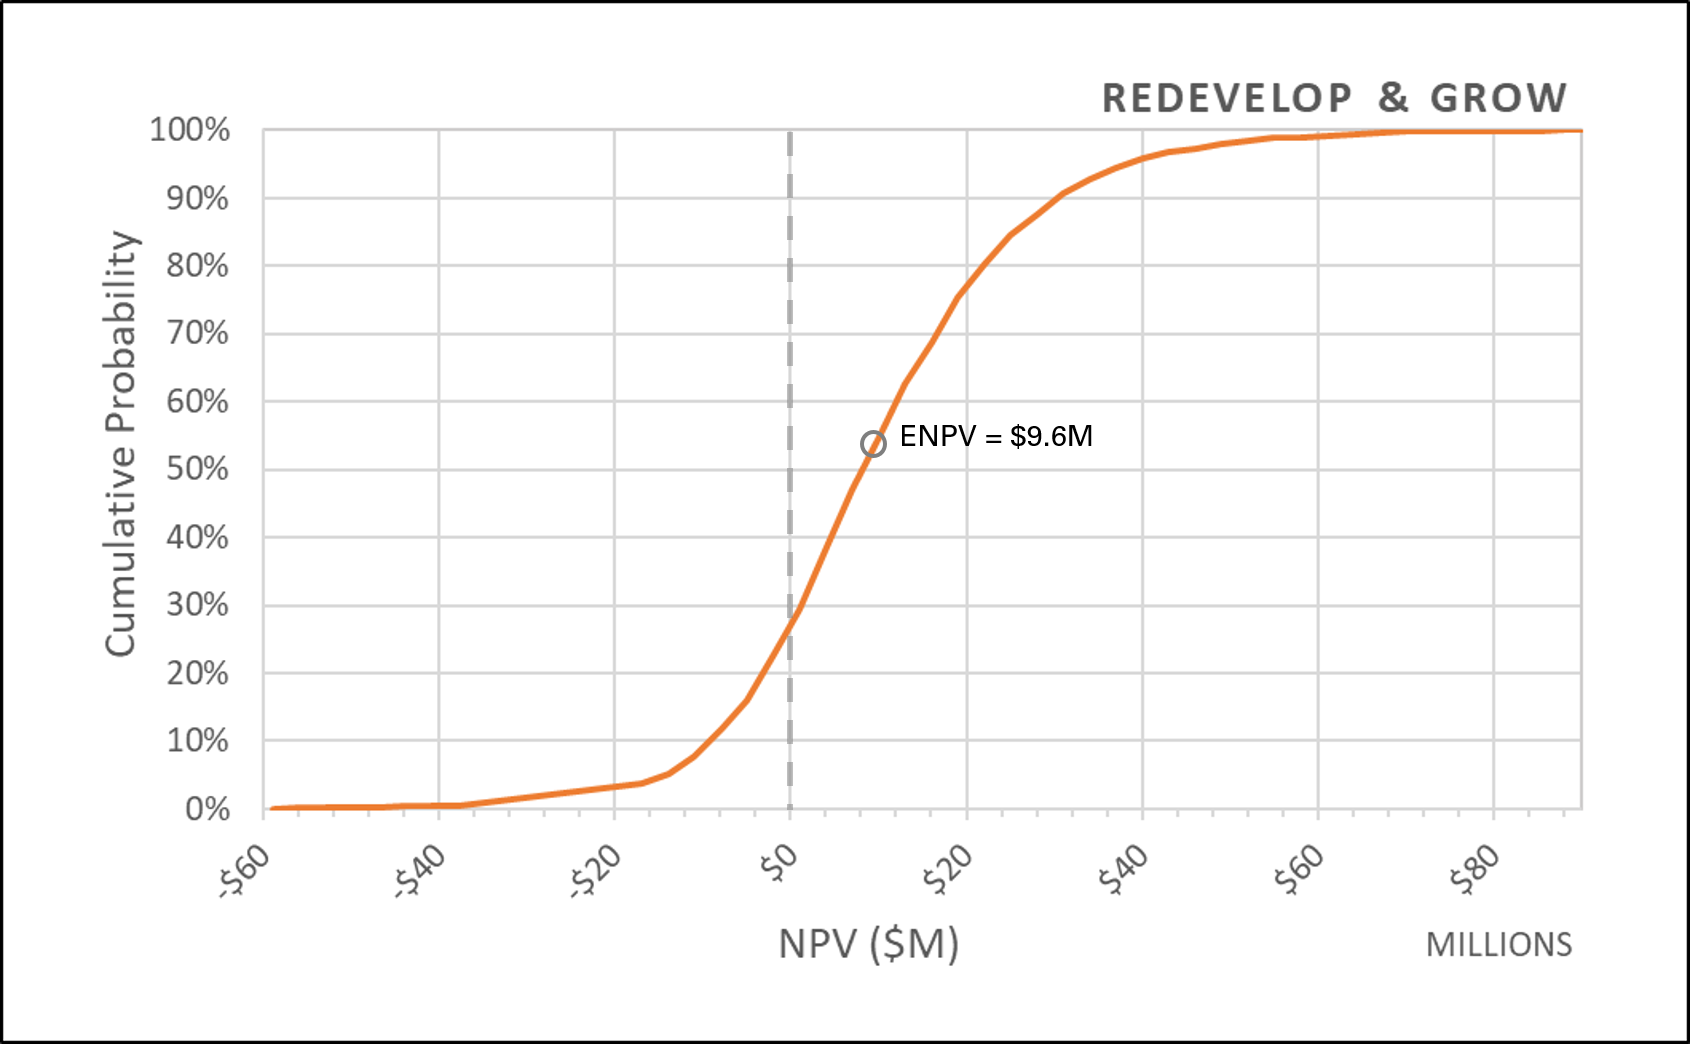
\includegraphics[width=.85\textwidth]{templates/images/Figure-Grow_Case_CDF.png}
\caption[Probabilistic Redevelop \& Grow Case CDF]{Cumulative distribution function for the Redevelop \& Grow Case probabilistic cost model. The curve summarizes results from 2000 model realizations. NPV is reported in \$M, where M is million.}
\label{fig:grow_case_cdf}
\end{figure}

Some caution should be taken in applying learnings from this model to a real-world geothermal project. Results here depend on a few important assumptions, including the willingness of a partner utility company to accept capacity increases above the market rate for electricity on any given year, the direct relationship between large price increases and electricity demand, and the overall monotonic increase in electricity prices over time. With regard to the latter, the price model used in this analysis includes a single step change and annual volatility (see Figure \ref{fig:elec_price_prob}), but other forecasts exist that depict negative year-on-year trends not modeled here \citep{murphy_electrification_2021}. As discussed in Section \ref{ch4:future_elec}, the interactions between different energy markets and dynamics of major events like future electrification are complex, worth considering, and beyond the scope of this thesis. 

\subsection{Summary Statistics}
\label{ch6:grow_stats}

Table \ref{tab:grow_stats} outlines key statistical measures summarizing the performance of the Redevelop \& Grow Case probabilistic cost model.

\begin{table}[H]
\centering
\begin{tabular}{|l|r|}
\hline
\textbf{Redevelop \& Grow Case Statistics} & N=2000 \\ \hline
ENPV & \$9.6M \\ \hline
STD(NPV) & \$16.5M \\ \hline
P05 NPV & -\$14.2M \\ \hline
P50 NPV & \$8.2M \\ \hline
P95 NPV & \$38.2M \\ \hline
\% Difference from NPV$_{s}$ & 832\% \\ \hline
\end{tabular}
\caption[Redevelop \& Grow Case statistics]{Redevelop \& Grow case model statistics for 2000 model realizations. NPV is reported in \$M, where M is million. NPV$_s$ refers to the static model NPV, as reported in Table \ref{tab:static_mod_stats}.}
\label{tab:grow_stats}
\end{table}

\section{Full Flexibility Case Probabilistic Model}

\subsection{Model Results}
\label{ch6:reduce_results}

\begin{figure}[!htp]
\centering
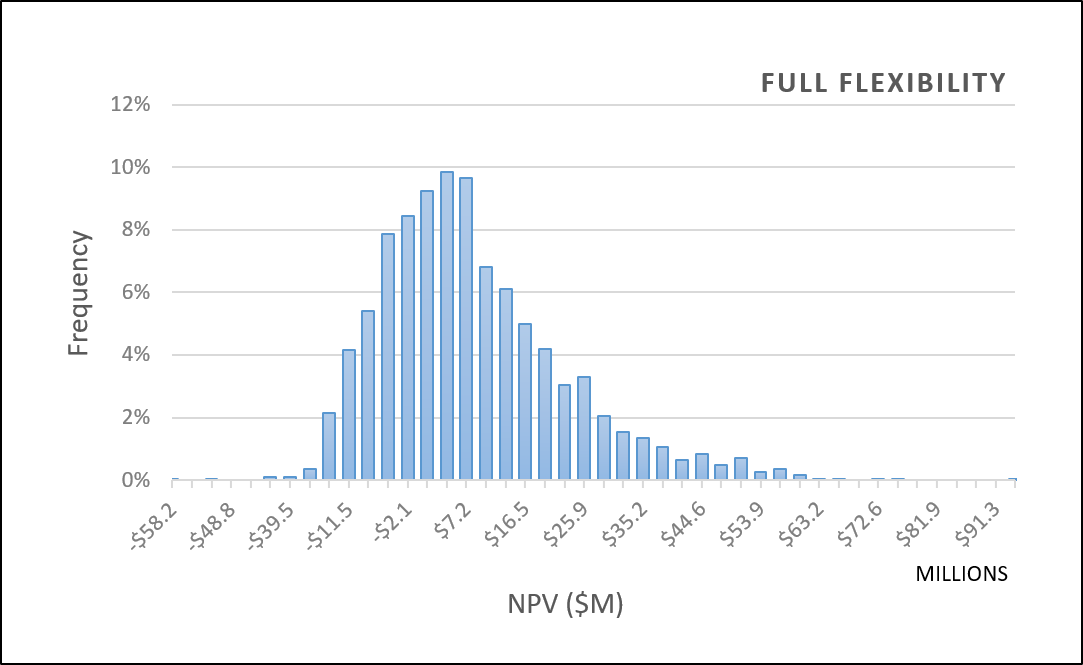
\includegraphics[width=.85\textwidth]{templates/images/Figure-Reduce_Case_Histogram.png}
\caption[Full Flexibility Case histogram]{CAPTION}
\label{fig:reduce_case_hist}
\end{figure}

\begin{figure}[!htp]
\centering
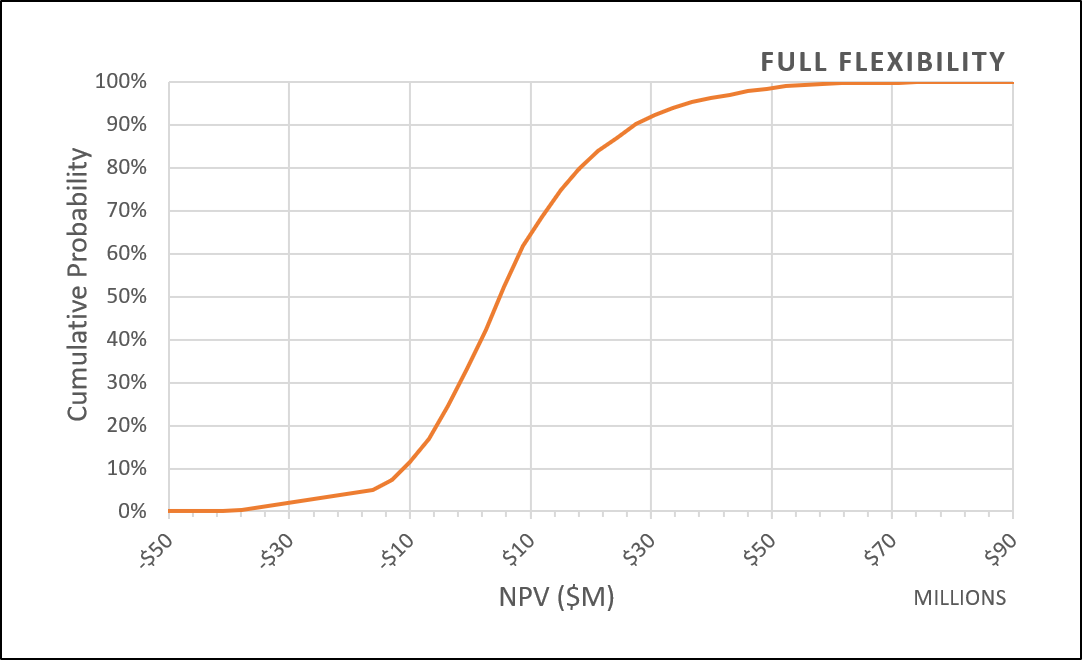
\includegraphics[width=.85\textwidth]{templates/images/Figure-Reduce_Case_CDF.png}
\caption[Full Flexibility Case CDF]{CAPTION}
\label{fig:reduce_case_cdf}
\end{figure}

\subsection{Summary Statistics}
\label{ch6:reduce_stats}

\begin{table}[H]
\centering
\begin{tabular}{|l|r|}
\hline
\textbf{Full Flexibility Case Statistics} & N=2000 \\ \hline
ENPV & \$6.7M \\ \hline
STD(NPV) & \$16.0M \\ \hline
P05 NPV & -\$16.3M \\ \hline
P50 NPV & \$4.9M \\ \hline
P95 NPV & \$36.2M \\ \hline
\% Difference from NPV$_{s}$ & 545\% \\ \hline
\end{tabular}
\caption[Full Flexibility Case statistics]{Full Flexibility case model statistics for 2000 model realizations. NPV is reported in \$M, where M is million. NPV$_s$ refers to the static model NPV, as reported in Table \ref{tab:static_mod_stats}.}
\label{tab:reduce_stats}
\end{table}

\section{Full Flexibility Sensitivity Testing}
\label{ch6:sensitivity}

\begin{figure}[!htp]
\centering
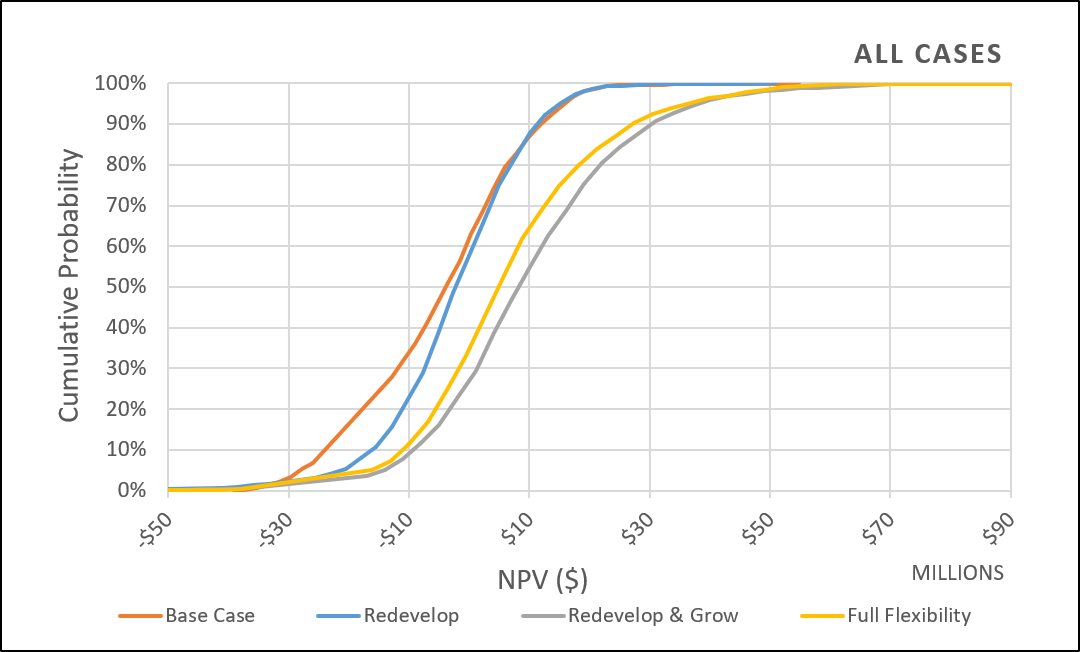
\includegraphics[width=.85\textwidth]{templates/images/Figure-All_Case_CDF.png}
\caption[All Cases CDF]{CAPTION}
\label{fig:all_case_cdf}
\end{figure}

\subsection{Reduction Amount}
\label{ch6:sens_redamt}

\begin{figure}[!htp]
\centering
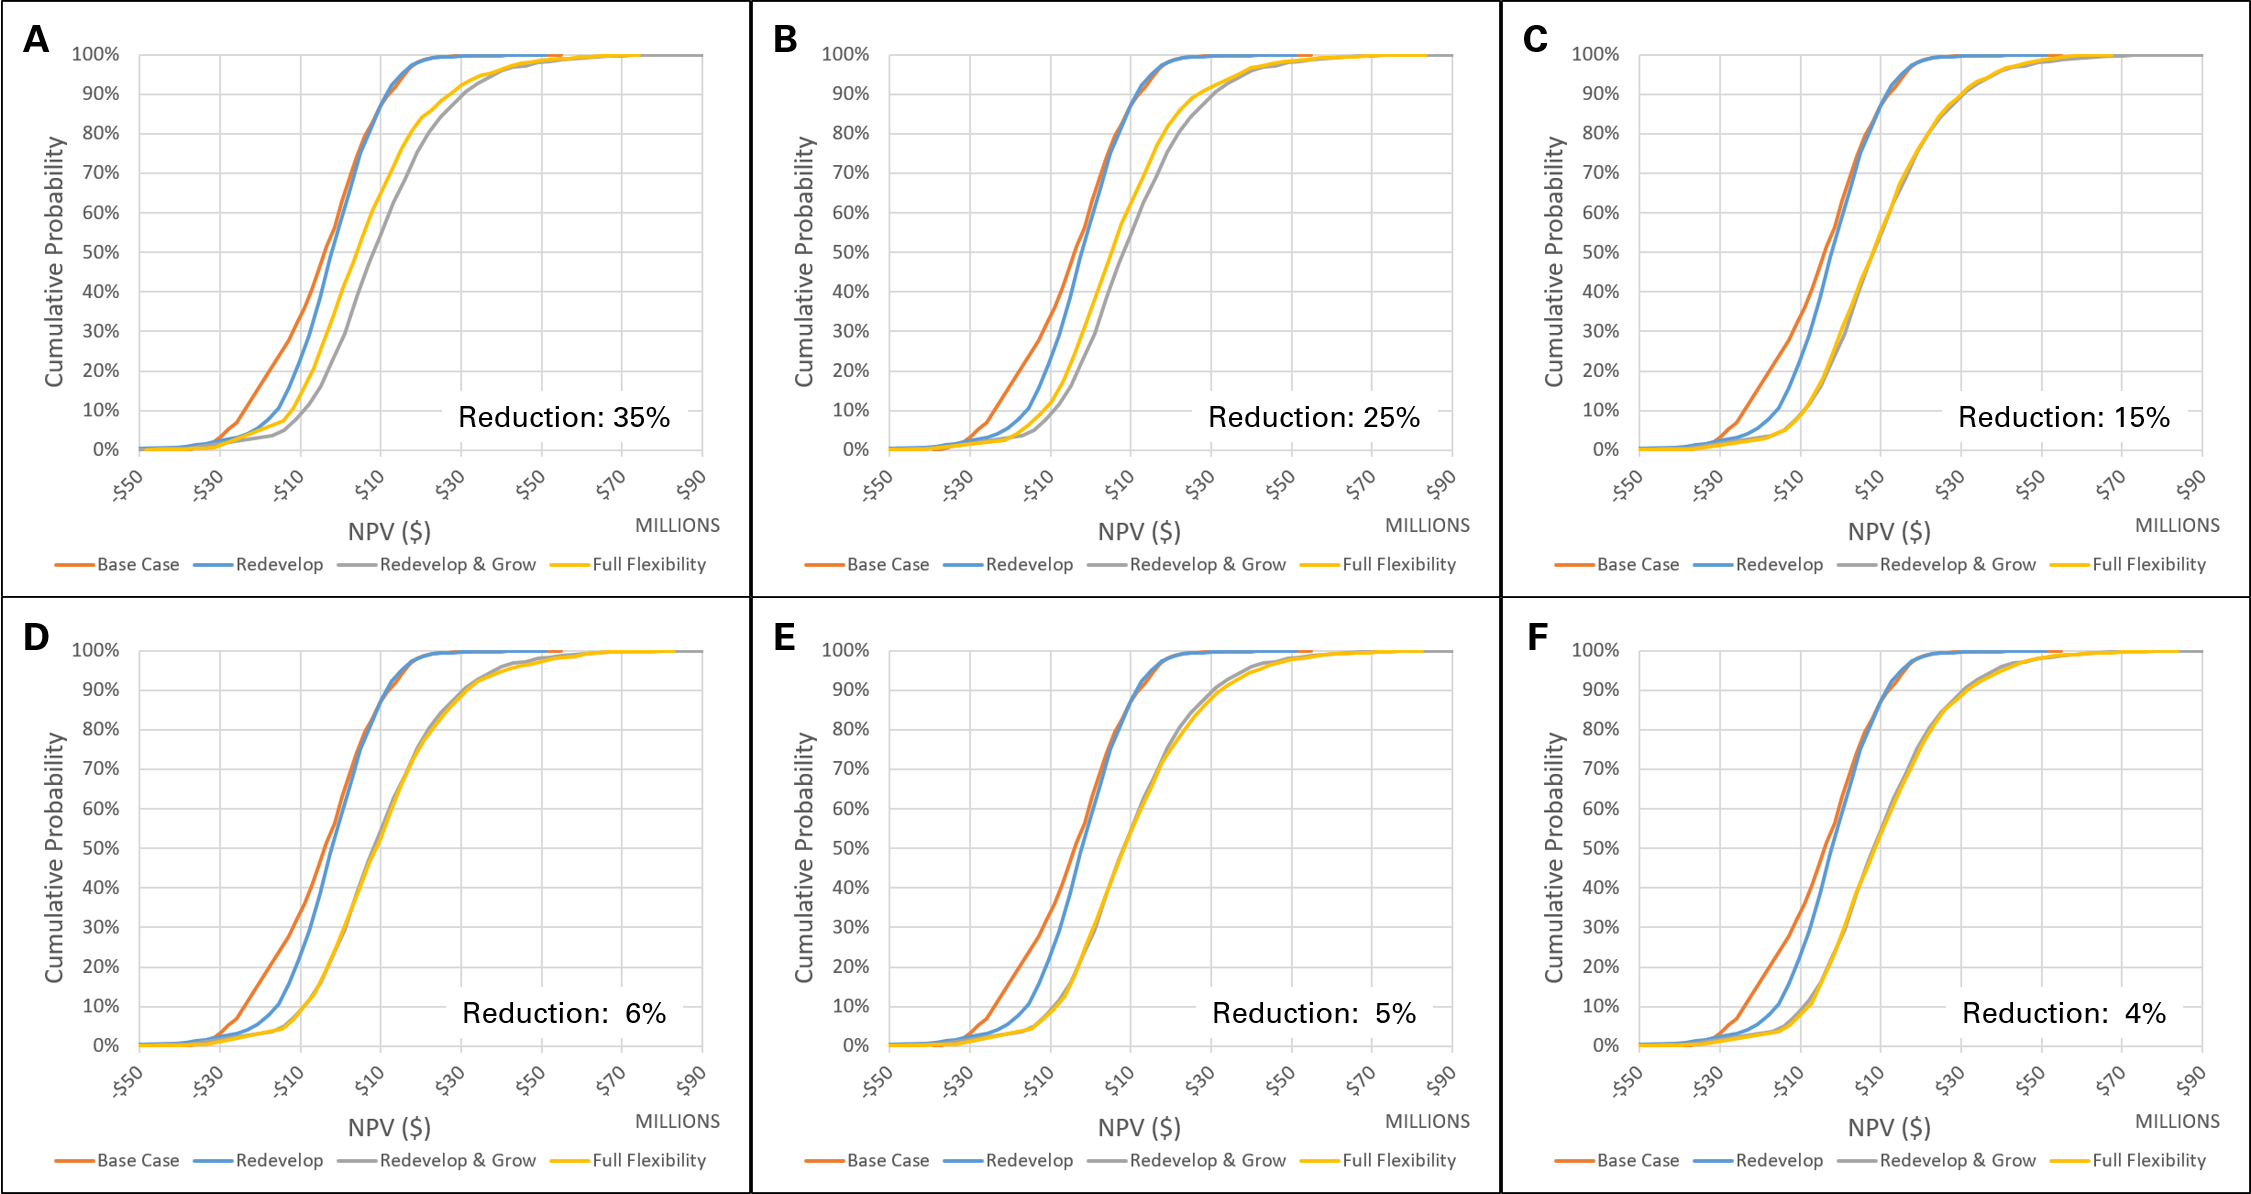
\includegraphics[width=.98\textwidth]{templates/images/Figure-Sensitivity_Reduction.pdf.png}
\caption[Reduction Amount sensitivity test]{Reduction Amount sensitivity test}
\label{fig:sens_test_reduction}
\end{figure}

\subsection{Expansion Amount}
\label{ch6:sens_expamt}

\begin{figure}[!htp]
\centering
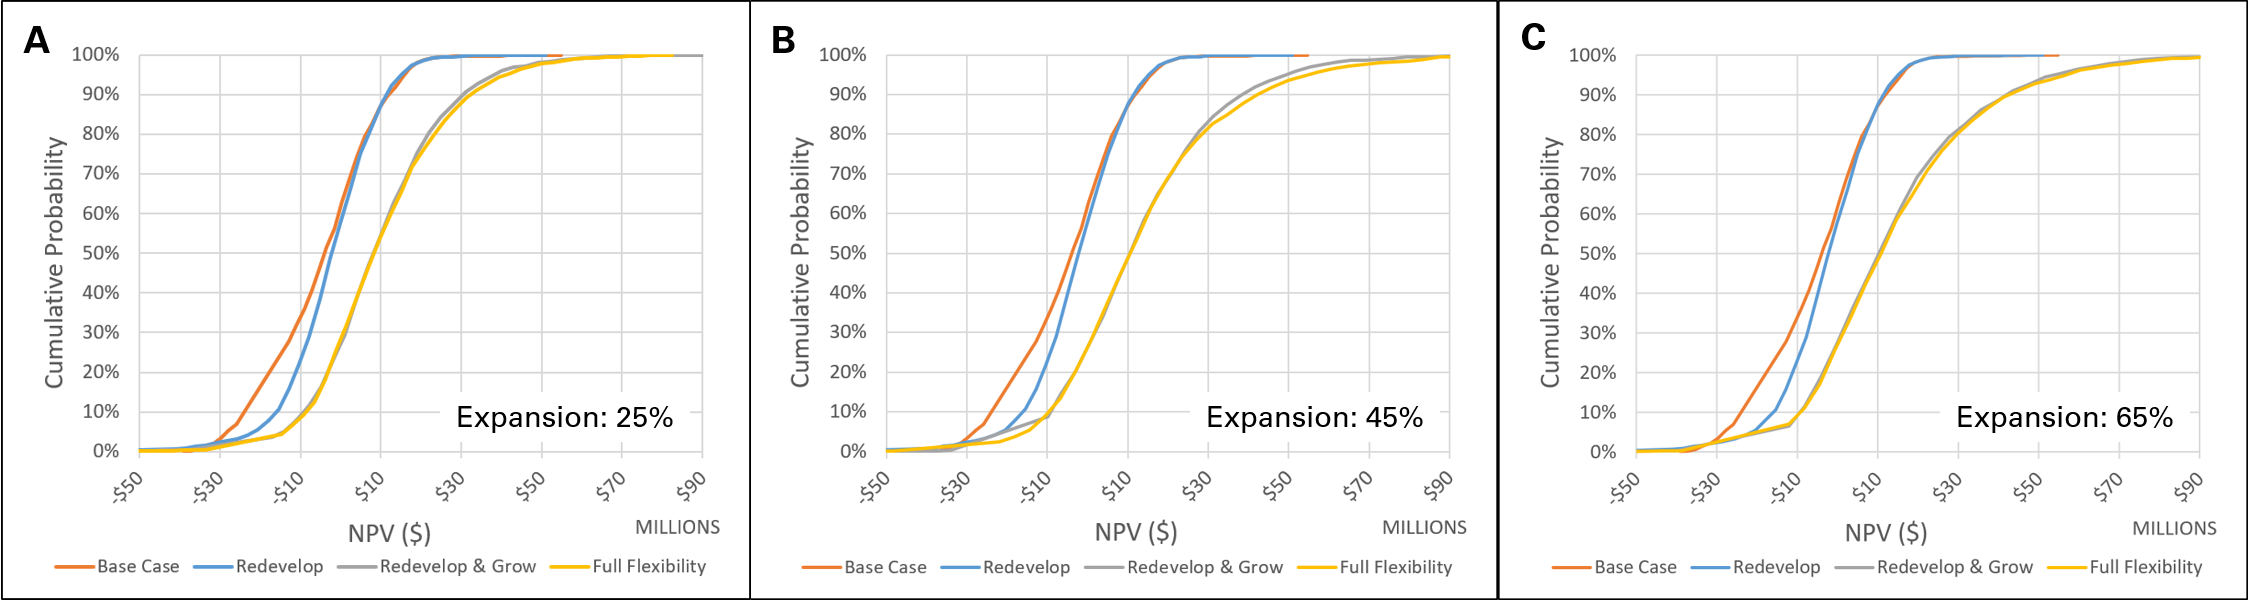
\includegraphics[width=.98\textwidth]{templates/images/Figure-Sensitivity_Expansion_Amount.png}
\caption[Expansion Amount sensitivity test]{Expansion Amount sensitivity test}
\label{fig:sens_test_expansion}
\end{figure}

\section{Recap}